\clearpage 
\section{Discussion}
\label{sec:discussion}

One observation that can be made from the experiments in the previous sections is that \textbf{admissible \astar
can be seen as a series of satisficing searches on each plateau}. In this view, the problem of tiebreaking can be
reduced to a satisficing search.

Our notion of \emph{admissible sorting strategy} dictates that the
search within the same $f$ plateau can be an arbitrary satisfiable search. For example,
if we ignore the first sorting criterion in the standard admissible strategy
$[f,h,\fifo]$, we get $[h,\fifo]$, which is exactly
the same configuration as a GBFS using \fifo default tiebreaking. It
means that within the plateau of the same $f$, $[f,h,\fifo]$ is
performing a satisficing GBFS.
As another example, the reason for the poor performance of $[f,\fifo]$
is clearly that it is running $[\fifo]$,
an uninformed satisficing breadth-first search in the plateau.
Furthermore, the good performance of $[f^{\lmcut},\ffo,\fifo]$ is also clear:
$\ffo$ is by itself known to be a \sota inadmissible heuristic
function for satisficing GBFS, and 
if we ignore the first sorting criterion, $[f^{\lmcut},\ffo,\fifo]$ is a GBFS with $[\ffo,\fifo]$.

Now, we reinterpret \astar as follows: \astar expands the nodes in a best-first order of $f$ value. When the
heuristic function is admissible, $f$ value of the nodes expanded by \astar never decreases during the
search process.
Thus, the entire process of \astar can be considered as a series of blocks of search on each $\plateau{f}$.
The search in each plateau terminates when the plateau is proven to contain no goal nodes (UNSAT), or some goal is found (SAT).
When the plateau is UNSAT, then the search continues to the plateau with the next least $f$ value.

\begin{figure}[htbp]
 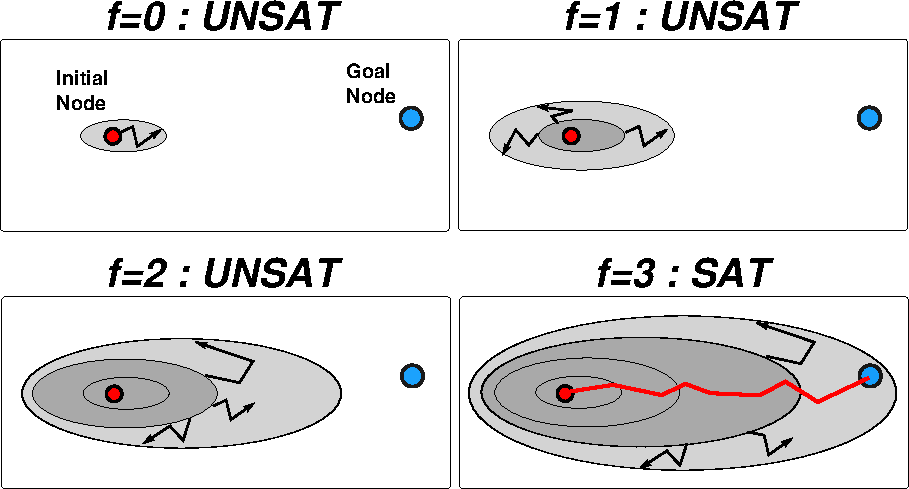
\includegraphics{img/astar/plateau-5.pdf}
 \caption{Concept of \astar as sequence of satisficing searches.}
\end{figure}

Similar concept is common in SAT/IP model-based sequential / temporal planning
\cite{rintanen2012planning,van2005optiplan}, but in a slightly different sense.  In model-based planning, a
planning problem is converted to a corresponding constraint satisfaction problem with a finite horizon $t$ (plan
length / makespan). The search starts from the horizon 0 and tests if the problem is satisfiable. If not, then it
increases the horizon and retests the same problem with additional constraints for a new horizon $t+1$. In the
forward heuristic search such as \astar, the concept of horizon corresponds to the $f$ value, which is a lower
bound of the solution cost.

The key difference in the \astar-based optimal planning from the model-based planning is
that the information is transmitted between different horizons:
In \astar, nodes that are generated in the smaller
$f$ layer will be ``sent'' to the larger $f$ layer through the global OPEN
list, while the current model-based methods prove the satisfiability of
different horizons independently -- in each iteration of the search,
they have to generate a new instance of a SAT/IP problem, and the
underlying model-based solvers are forced to start the search from the scratch.

More precisely, each iteration of \astar only requires to test the satisfiability in the space of particular
$f$ while each iteration of model-based solvers tests the satisfiability in the space of all nodes $0<f(n)<t$
($t$ is a horizon).  This latter behavior also connects model-based approaches to Iterative Deepening \astar
\cite{korf1985depth} where the search is restarted from the scratch on each iteration, forgetting the past search
effort in order to ensure the linear space usage.
% 
\todo*{A more standard interpretation of the connectin between SAT/IP/CSP planning vs A* is that SAT/IP/CSP are
doing iterated deepening, where each iteration seeks a satisficing solution, like IDA*. }
% 
\todo*{In fact, exploring the application of ``IDA* = series of satisficing seraches'' seems like an interesting
direction for future work, e.g., how to simulate depth-based tiebreaking (node ordering) in IDA*? IDA* is useful
for domains where memory limitations are the bottleneck, so keeping the depth buckets in memory may not be
possible. More broadly, linear space, best-first search including RBFS}

\begin{figure}[htbp]
 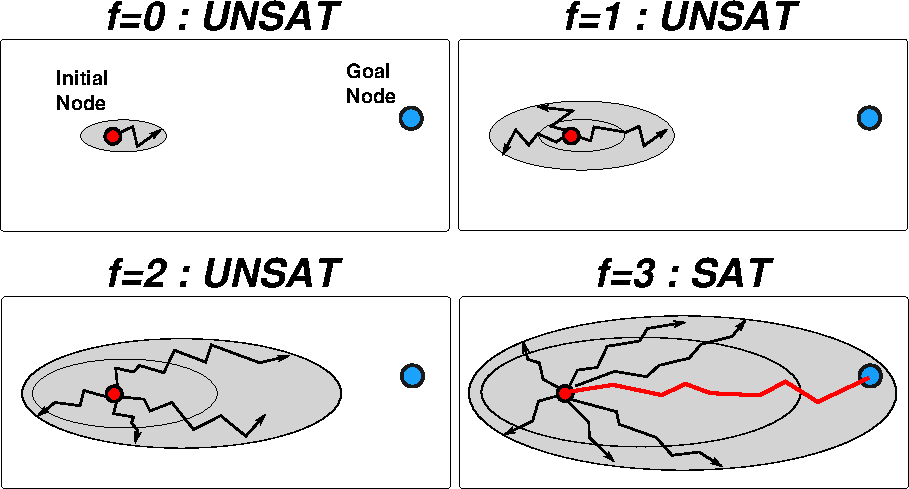
\includegraphics{img/astar/plateau-6.pdf}
 \caption{Concept of IDA* as sequence of satisficing searches.}
\end{figure}

One may notice that there is a difference between the satisficing search and the search on a plateau that
the former starts from a single initial node while the latter may start from multiple initial nodes.
For example, in satisficing planning, the search space usually contains a single start node which corresponds to an initial or the current state in the real world.
% 
In contrast, when \astar starts expanding a new current $f$ value $f_{\mit{cur}}$ after expanding all nodes with $f<f_\mit{cur}$,
there may be multiple nodes with $f=f_\mit{cur}$ in the open list.
These nodes are generated as a result of expansions of the parent nodes with $f<f_\mit{cur}$.
% The search in this plateau terminates when the plateau is proven to contain no goal nodes (UNSAT), or some goal is found (SAT).
% When the plateau is UNSAT, then the search continues to the next plateau.
% 
However, this difference is superficial because the latter can be reduced to the former case by introducing a dummy
node to a graph which acts as a common parent of all initial nodes, and reformulate the problem as the search
starts from this dummy node.

This entire view shows an interesting direction for future work.
Although we evaluated only one \sota satisficing configuration $\ffo$ in
the experiments, it does not prevent us from applying yet
more variety of satisficing planning techniques to the tiebreaking in optimizing search.
There are plenty of candidates: Lazy evaluation \cite{richter2010lama}, Alternating/Pareto open
list \cite{RogerH10}, helpful actions (preferred operators) \cite{Hoffmann01},
random walk local search \cite{nakhost2009monte}, macro operators
\cite{Botea2005,ChrpaVM15}, factored planning
\cite{amir2003factored,brafman2006factored,Asai2015} and
exploration-based search enhancements
\cite{valenzano2014comparison,xie14type,Valenzano2016}.


\subsection{Depth Diversification for Satisficing Search}

However, how promising is this view, or hypothesis, actually?
In order to strengthen the connection between tiebreaking and satisficing search,
we conducted another set of experiments. In the previous experiments, we showed that the distance-to-go
\ff heuristic $\ffo$ for \textbf{satisficing search within a plateau} was improved by the depth diversification
$\depth$.
% 
A natural extension to this idea is that the depth metric could also enhance the performance of $\ffo$ used for
\textbf{satisficing search in general}, which should hold if the search on plateaus is a satisficing search.
% 
% Our claim is that this \emph{should} work if our observation is correct, and if it is, it becomes another
% testimonial that our future direction (importing satisficing techniques to optimal search) is promising.
% This is different from a simple claim like ``X worked in optimizing search, so it should also work in satisficing search''.
\todo*{``exporting from optimizing to satisficing'' and ``exporting from satisficing to optimizing'' are not symmetric. The latter is interesting and surprising, the former, not so much. --- changed the tone, emphasized the purpose}

We provide preliminary results on the 280 IPC8 satisficing track
instances. We tested GBFS using the distance-to-go variations of three
\sota inadmissible heuristics for satisficing search: FF heuristics
 \cite{Hoffmann01}, Causal Graph (CG) heuristics \cite{Helmert2006} and
Context Enhanced Additive (CEA) heuristics\ \cite{helmert2008unifying}.
For each heuristics, we tested eager and lazy search, with and without
the depth metric.  Tests are conducted under 5 min, 4GB
resource constraint.

In Eager search, depth metric
improved the performance of $\cgo$ ($60\rightarrow $ \textbf{64}), but no
improvement was observed in $\ceo$ ($62\rightarrow 62$)
and $\ffo$ ($73\rightarrow 73$). In Lazy search, depth metric
improved the performance of all three heuristics
($\cgo$: $36\rightarrow $ \textbf{50}, 
 $\ceo$: $39\rightarrow $ \textbf{48}, 
 $\ffo$: $54\rightarrow $ \textbf{93}). This is reasonable
because lazy search forces each node to derive the heuristic value from
its parent, and it makes more nodes to have the same heuristic value,
increasing the size of a plateau.

% \begin{table}[htbp]
%  \setlength{\tabcolsep}{0.3em}
%  \centering
%  \def\header{&\multicolumn{6}{c|}{Eager Search}&\multicolumn{6}{c|}{Lazy Search}\\}

\begin{center}
\begin{tabular}{|r|*{2}{*{3}{cc|}}}
\header & \(\ceo\) & \(\ceo\) & \(\cgo\) & \(\cgo\) & \(\ffo\) & \(\ffo\) & \(\ceo\) & \(\ceo\) & \(\cgo\) & \(\cgo\) & \(\ffo\) & \(\ffo\)\\
 & g & G & g & G & g & G & g & G & g & G & g & G\\
\hline
IPC8 & 62 & 62 & 60 & \textbf{64} & 73 & 73 & 36 & \textbf{50} & 39 & \textbf{48} & 54 & \textbf{93}\\
\hline
\end{tabular}
\end{center}

%  \caption{
%  Coverages under 5 min, 4GB experiments, comparing the variants with
%  and without depths. All configurations uses \fifo default
%  tiebreaking (we omit it from the description below).
%  $\ffo,\ceo,\cgo$ are the distance-to-go variations of FF,
%  Context Enhanced Additive, Causal Graph heuristics.
%  (g): GBFS with $[\hh]$ sorting strategy.
%  (G): GBFS with depth based diversification $[\hh,\depth]$.
%  }
%  \label{tbl:gbfs}
% \end{table}

% We also tested each combination on Type-GBFS, a recent \sota enhancement
% to GBFS. The results in \reftbl{tbl:type-gbfs} show that the depth
% metric also improves the performance of these configurations. Furthermore, we tested LAMA and
% Type-LAMA with and without depth metric. LAMA is an old \sota
% satisficing planner combining various satisficing enhancements such as
% Lazy-evaluation, distance-to-go estimates, multi-heuristic search and
% preferred operator queues. Type-LAMA is a newer \sota planner and an
% extension of LAMA using Type-GBFS, and it has performed the best among non-portfolio
% planners in IPC8 satisficing track. In \reftbl{tbl:lama}, we observed
% that the depth metric also improved the performance of LAMA and Type-LAMA.
% 
% \begin{table}[htbp]
%  \setlength{\tabcolsep}{0.3em}
%  \centering
%  \def\header{&\multicolumn{6}{c|}{Eager Search}&\multicolumn{6}{c|}{Lazy Search}\\}

\begin{center}
\begin{tabular}{|r|*{2}{*{3}{cc|}}}
\header & \(\ceo\) & \(\ceo\) & \(\cgo\) & \(\cgo\) & \(\ffo\) & \(\ffo\) & \(\ceo\) & \(\ceo\) & \(\cgo\) & \(\cgo\) & \(\ffo\) & \(\ffo\)\\
 & gt & Gt & gt & Gt & gt & Gt & gt & Gt & gt & Gt & gt & Gt\\
\hline
IPC8 & \textbf{57} & 55 & 76 & \textbf{79} & 80 & 79 & 44 & \textbf{53} & 66 & \textbf{74} & 66 & \textbf{92}\\
\hline
barman(20) & 0 & 0 & 0 & 0 & \textbf{4} & 2 & 0 & 0 & 0 & 0 & 0 & 0\\
cavediving(20) & 6 & 6 & 7 & 7 & 7 & 7 & 6 & 7 & 7 & 8 & 7 & 7\\
childsnack(20) & \textbf{2} & 0 & \textbf{3} & 0 & 0 & 0 & 2 & 1 & 6 & 5 & 2 & 2\\
citycar(20) & 4 & 5 & 1 & 1 & 3 & 3 & 1 & \textbf{9} & 0 & 0 & 0 & \textbf{7}\\
floortile(20) & 2 & 2 & 2 & 2 & 2 & 2 & 2 & 2 & 1 & 1 & 2 & 2\\
GED(20) & 0 & 0 & 8 & 9 & 16 & 15 & 0 & 0 & 11 & 11 & 15 & \textbf{17}\\
hiking(20) & 16 & 16 & 20 & 20 & 20 & 20 & 16 & 15 & 18 & 19 & 18 & 18\\
maintainance(20) & 16 & 16 & 16 & 16 & 13 & 13 & 7 & 7 & 7 & 7 & 9 & 10\\
openstacks(20) & 0 & 0 & 0 & 0 & 0 & 0 & 0 & 0 & 0 & 1 & 0 & \textbf{6}\\
parking(20) & 0 & 0 & 0 & 0 & 1 & 2 & 0 & 0 & 0 & 0 & 1 & \textbf{8}\\
tetris(20) & 1 & 1 & 13 & \textbf{15} & 2 & 2 & 1 & 3 & 9 & \textbf{15} & 2 & \textbf{4}\\
thoughtful(20) & 9 & 8 & 5 & 5 & 12 & 13 & 9 & 9 & 5 & 5 & 10 & 11\\
transport(20) & 1 & 1 & 1 & \textbf{4} & 0 & 0 & 0 & 0 & 2 & 2 & 0 & 0\\
visitall(20) & 0 & 0 & 0 & 0 & 0 & 0 & 0 & 0 & 0 & 0 & 0 & 0\\
\hline
\end{tabular}
\end{center}

%  \caption{
%  Coverages of Type-GBFS under 5 min, 4GB experiments, comparing the variants with
%  and without depths. All configurations uses \fifo default
%  tiebreaking (we omit it from the description below).
%  $\ffo,\ceo,\cgo$ are the distance-to-go variations of FF,
%  Context Enhanced Additive, Causal Graph heuristics.
%  In each expansion, Type-GBFS alternates standard GBFS and Type-based exploration using $[g,\hh]$.
%  The sorting strategy of the GBFS part of (gt) is $[\hh]$, while (Gt) uses $[\hh,\depth]$.
%  }
%  \label{tbl:type-gbfs}
% \end{table}
% 
% \begin{table}[htbp]
%  % \setlength{\tabcolsep}{0.1em}
%  \centering
%  \begin{center}
\begin{tabular}{|r|ll|ll|}
 &  &  &  & \\
 & LAMA & LAMA & Type-LAMA & Type-LAMA\\
 &  & + depth (\(\ffo\)) &  & + depth (\(\ffo\))\\
\hline
IPC8 & 111 & \textbf{125} & 112 & \textbf{117}\\
\hline
barman(20) & 8 & \textbf{10} & 9 & 8\\
cavediving(20) & 7 & 7 & 6 & 7\\
childsnack(20) & 0 & \textbf{10} & 2 & \textbf{6}\\
citycar(20) & 1 & 0 & 5 & 4\\
floortile(20) & 2 & 2 & 2 & 2\\
GED(20) & 20 & 20 & 20 & 20\\
hiking(20) & 15 & \textbf{17} & 15 & 15\\
maintainance(20) & 1 & 1 & 6 & 6\\
openstacks(20) & 17 & 17 & 15 & \textbf{17}\\
parking(20) & 9 & 9 & 6 & 6\\
tetris(20) & 2 & 2 & 2 & 1\\
thoughtful(20) & 14 & 15 & 14 & 15\\
transport(20) & 2 & 2 & 1 & \textbf{3}\\
visitall(20) & 13 & 13 & \textbf{9} & 7\\
\hline
\end{tabular}
\end{center}

%  
%  \caption{ Coverages of satisficing planners LAMA (winner of IPC7, old \sota)
%  and Type-LAMA (non-portfolio winner of IPC8, newer \sota) under 5 min, 4GB
%  experiments, comparing the performance between the original and the
%  depth-enhanced variants. All configurations run the first GBFS
%  iteration only, apply \fifo default tiebreaking (we omit it from
%  the description below), apply lazy evaluation and use distance-to-go synergy
%  heuristics $\ffo / \hat{h}^{\text{LMcount}}$.
%  % 
%  LAMA alternates between four OPEN lists: an open list of $[\ffo]$, a
%  preferred operator queue of $\ffo$, an open list of
%  $[\hat{h}^{\text{LMcount}}]$, and a preferred operator queue of
%  $\hat{h}^{\text{LMcount}}$.  In contrast, Type-LAMA alternates
%  between five OPEN lists: In addition to the 4 queues in LAMA, it has a
%  type-based exploration queue using $[g,\ffo]$.  The depth is applied
%  only to the first queue, i.e. $[\ffo] \rightarrow [\ffo,\depth]$, and
%  is not applied to the other queues. In both LAMA and Type-LAMA, depth
%  metric improves the coverage.}
%  \label{tbl:lama}
% \end{table}

In the past, optimizing search techniques and satisficing search techniques used to be developed rather separately, and there have been only a handful of knowledge migration between them, most of which are abstract ideas such as delete-relaxation, landmarks, causal graphs or pattern database.
Otherwise, the migration is unidirectional, in particular from optimizing to satisficing search, because it is easy or trivial to relax the optimality requirements.
% 
Our results and the new observation, \textbf{optimal search is a sequence of satisficing searches on each plateau},
open up a new opportunity to break this boundary.  We provided the fundamentals of how and why we can import
satisficing search techniques to the optimizing search (e.g. $\ffo$ heuristics in optimal search).  There is a
large avenue for future work in making a migration happen in this novel direction.

